\documentclass[amsmath,amssymb,notitlepage,11pt]{revtex4}
%\documentclass[12pt]{article}
\usepackage{graphicx}
\usepackage{bm}% bold math
\usepackage{multirow}
\usepackage{booktabs}
\usepackage{verbatim}
\usepackage{hyperref}
\usepackage{enumitem}
\hypersetup{pdftex,colorlinks=true,allcolors=blue}
\usepackage{hypcap}
\usepackage{wrapfig}
\usepackage[small,compact]{titlesec}
\setlist[enumerate]{itemsep=0mm}

\begin{document}
\title{CLAS12 Slow Controls Operations Manual - v2.1}
\date{\today}
\begin{abstract}
\end{abstract}

\maketitle
\tableofcontents
\newpage

\section{Overview}

\begin{wrapfigure}{l}{0.15\textwidth}\centering\vspace{1cm}
  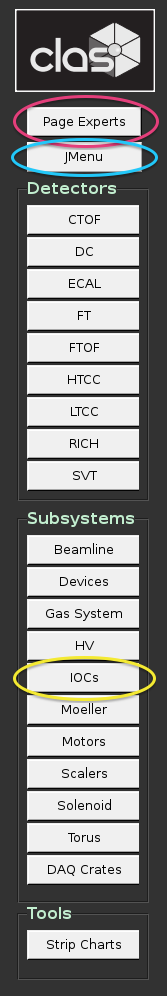
\includegraphics[width=0.15\textwidth]{pics/mainmenu}
  \caption{The main menu.\label{fig:mainmenu}}
\end{wrapfigure}

The operator interface for the Hall B controls systems is based on Control System Studio (also called CS-Studio or CSS) and allows access to all the necessary EPICS tools from a single application.  This system is accessible by user \texttt{clasrun} directly from all \texttt{clonpc\#\#} desktop computers in the Hall B Counting Room for shift workers (for remote access, see Section \ref{sec:remote}).


To start the control system with only the main menu as shown in Figure~\ref{fig:mainmenu}, in a terminal run: \begin{center}\texttt{clascss}\end{center}  This menu should normally already be open on all the neccessary desktops in the counting house.  The top portion of the menu is for specific detectors, while the bottom portion is for more general subsystems, and the most important parts for shift workers are described in the following sections.

\section{Alarms}

The user interface for the alarm handling system also runs in CS-Studio and includes visual and audible alarms.  Generally, \texttt{clonpc17} (with the two high monitors near the windowed doors) should always be running a full screen alarm handler.  To start the control system with the full alarm handler, in a terminal run:
\begin{center}\texttt{clascss-alarm}\end{center}
%{\em Before opening CS-Studio on a \texttt{clonpc} desktop in the counting house, check whether an instance is already running on that machine.  If one is, use that instance instead of opening another}.  
\begin{figure}[htpb]\centering
  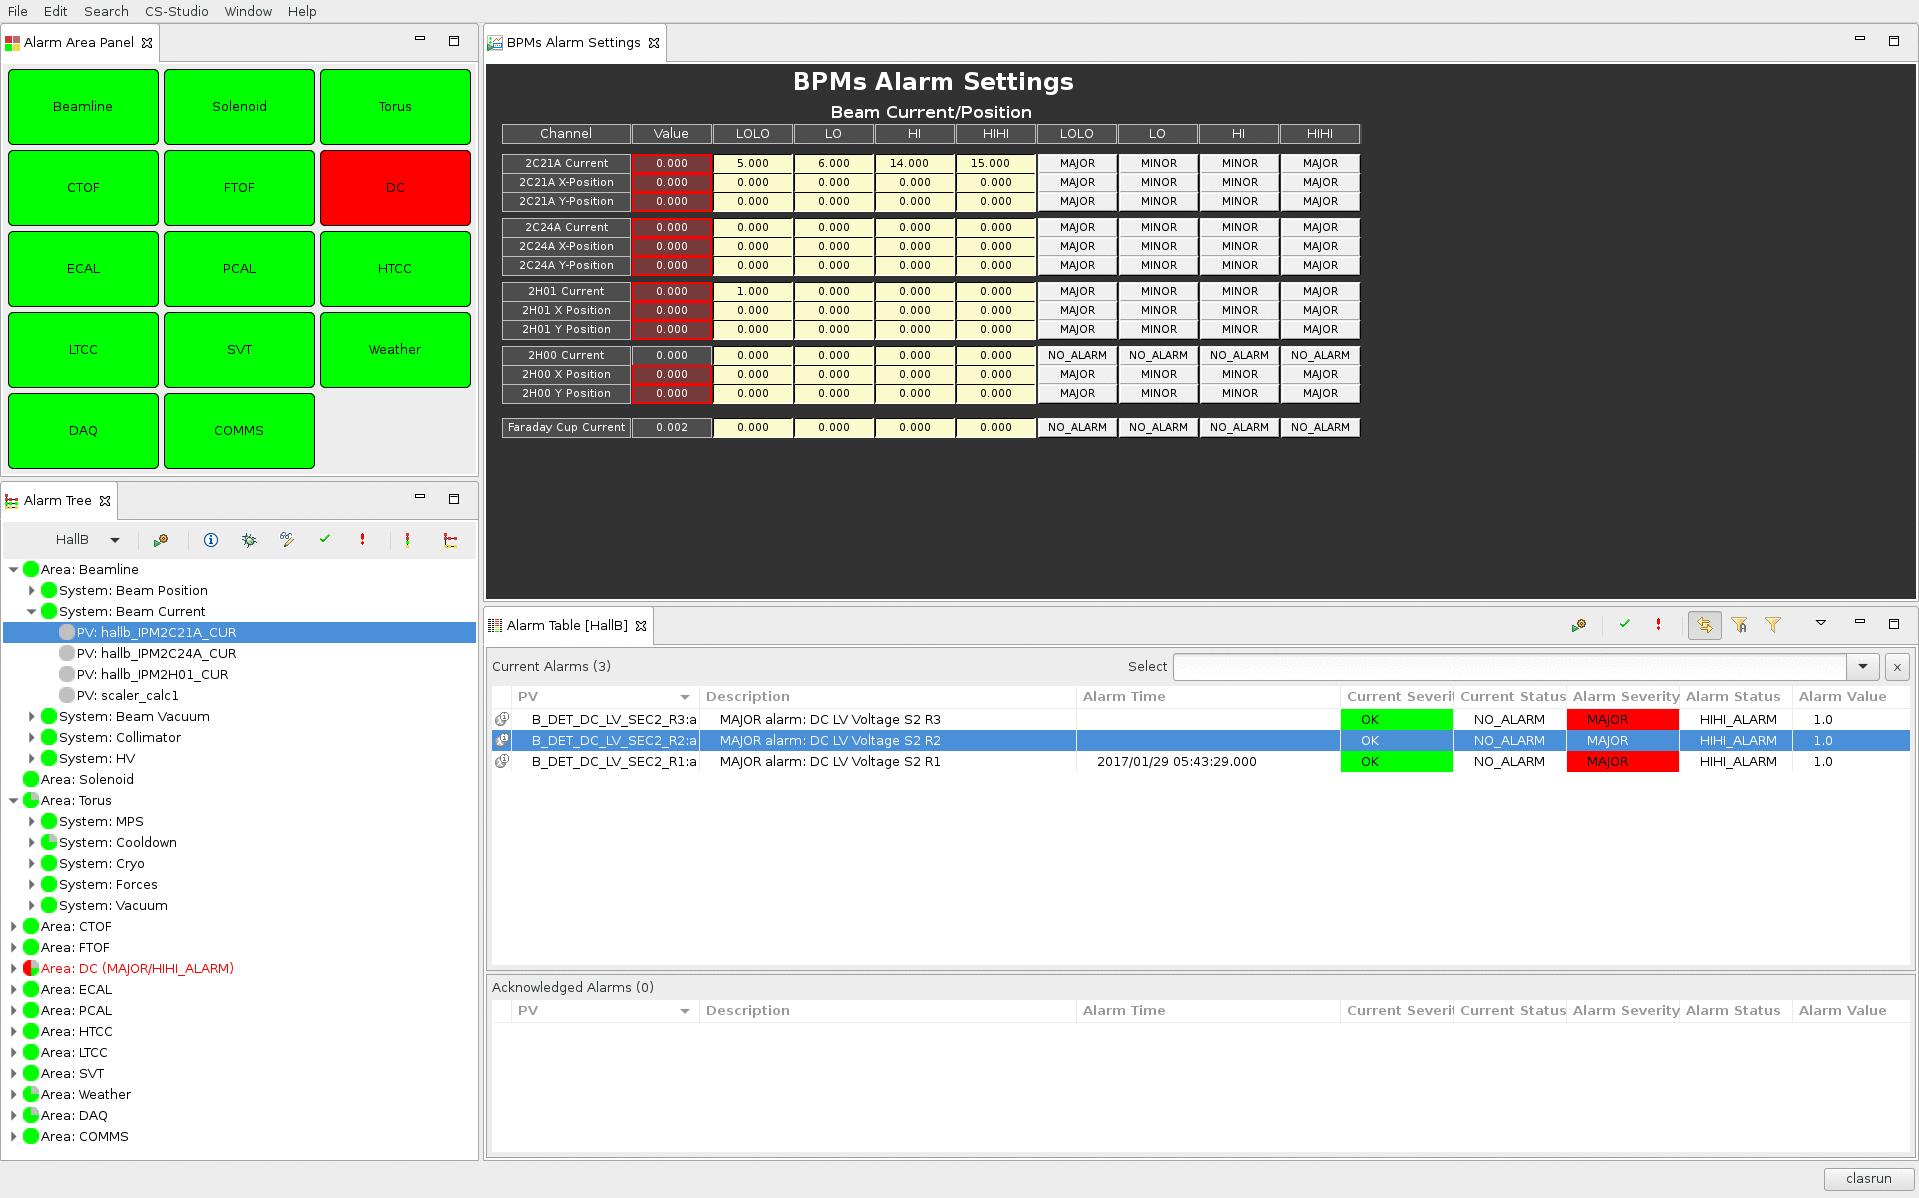
\includegraphics[width=0.99\textwidth]{pics/clas12alarm3}
  \caption{The alarm handling screen.\label{fig:alarmhandler}}
\end{figure}
The resulting window is shown in Figure~\ref{fig:alarmhandler} and contains the following sections:
\begin{enumerate}
    \item Top Left:  the {\em Area Panel}, an overview of the global alarm system status.  The color of the areas reflects the most severe alarm in that area.
    \item Bottom Left:  the {\em Alarm Tree}, a hierarchical view of all alarm settings.
    \item  Bottom Right:  the {\em Alarm Table} (see also Figure~\ref{fig:alarmtable}), containing a list of current alarms that need to be addressed and a separate list of already acknowledged alarms.
\end{enumerate}

When an alarm triggers, it will enter the {\em Alarm Table} and its color will change according to its severity.  The annunciator (running on \texttt{clonpc17}) will also audibly announce any new alarms or a count of currently active alarms.

By right-clicking on an alarm in the {\em Alarm Table}, a dropdown menu of actions is accessible (see Figure~\ref{fig:alarmguide}).  This dropdown list contains access to a {\em Guidance} screen with instructions that should be read and followed on how to deal with the specific alarm.  

The next step is to acknowledge the alarm using the {\em Acknowledge} option in the dropdown menu, which will silence the alarm and move it to the {\em Acknowledged Alarms} section until it is no longer in an alarm state.  

For many alarms there is also an option in the dropdown menu starting with {\em Open} that will open a screen necessary to address the specific alarm using the information from the {\em Guidance} screen.

\begin{figure}[htbp]\centering
  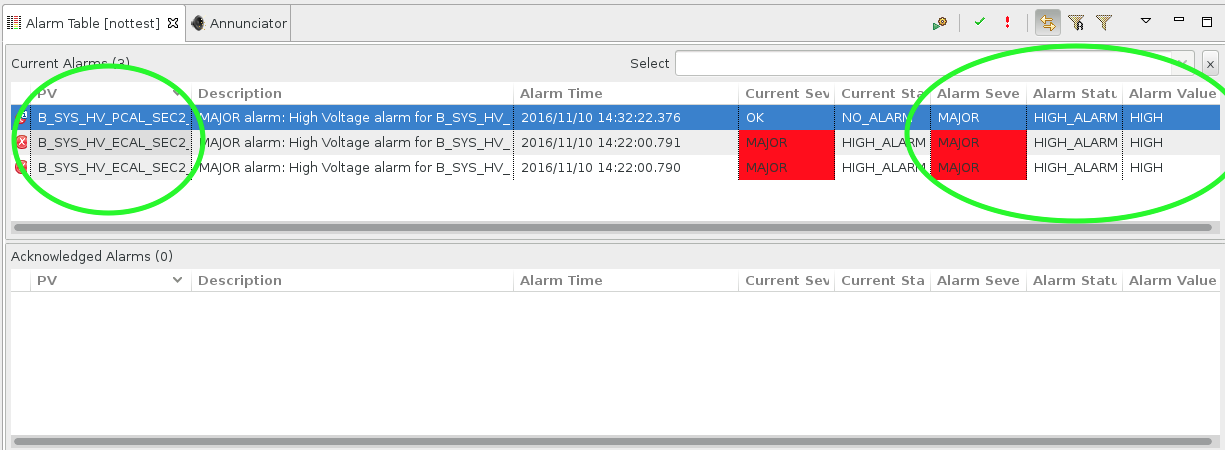
\includegraphics[width=0.99\textwidth]{pics/alarmtree}
  \caption{The {\em Alarm Tree} portion of the alarm screen, showing an example of three outstanding alarms to be addressed.  The first is no longer in an alarm state (denoted by the {\em OK} in the {\em Current Severity} column), and none of the three have been acknowledged (else they would have appeared instead in the lower {\em Acknowledged Alarms} section).\label{fig:alarmtable}}
\end{figure}
\begin{figure}[htbp]\centering
  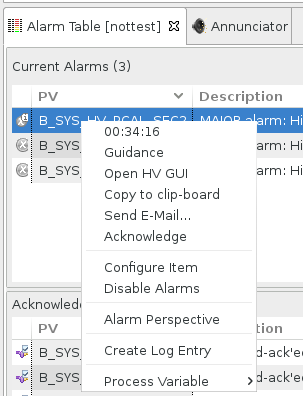
\includegraphics[width=0.3\textwidth]{pics/alarmguide}
  \caption{An example dropdown menu accessible by right-clicking on an alarm in the {\em Alarm Table}.  Important visible actions include a {\em Guidance} button, an {\em Open} screen action, and the {\em Acknowledge} action.  {\bf Note, the {\em Create Log Entry} item does not yet work} (see Section \ref{sec:logentry} instead).\label{fig:alarmguide}}
\end{figure}

\clearpage

\section{IOCs}
EPICS input-output controllers (IOCs) are the backend responsible for the actual communication with the hardware devices in the hall.  Figure~\ref{fig:iocmenu} illustrates access to the IOC controls screens from the main CLAS12 menu, as well as the overview IOC heartbeat screen.  The heartbeats should be flashing at 1 Hz for all IOCs, or else the IOC may be in need of reboot.  

\begin{figure}[htbp]\centering
  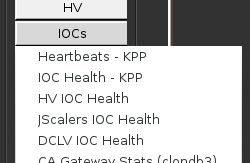
\includegraphics[width=0.25\textwidth]{pics/iocmenu-KPP}
  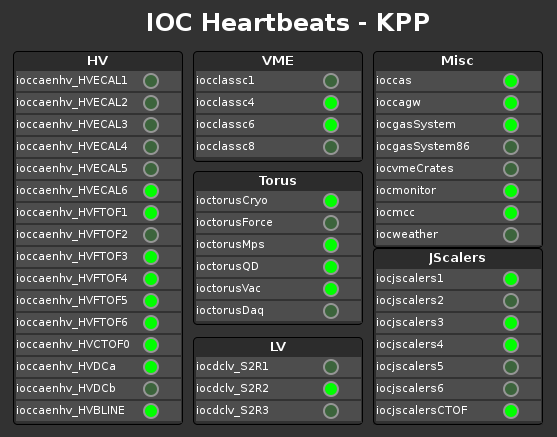
\includegraphics[width=0.65\textwidth]{pics/iocbeats-KPP}
  \caption{Dropdown menu (left) from the {\em IOCs} button in the main CLAS12 controls menu showing links to health screens for subsets of IOC groups, and the IOC heartbeat overview screen for the KPP Run (right).\label{fig:iocmenu}}
\end{figure}

By clicking on the IOC in the heartbeat screen (or the IOC health group in the main menu), controls to monitor and reboot the IOCs can be accessed, and an example is shown in Figure~\ref{fig:iochealth}.  Systems are in place to automatically start all necessary IOCs if for any reason they are not running (e.g. recovery from a power outage), however occaisonally a manual reboot is required.

\begin{figure}[htbp]\centering
  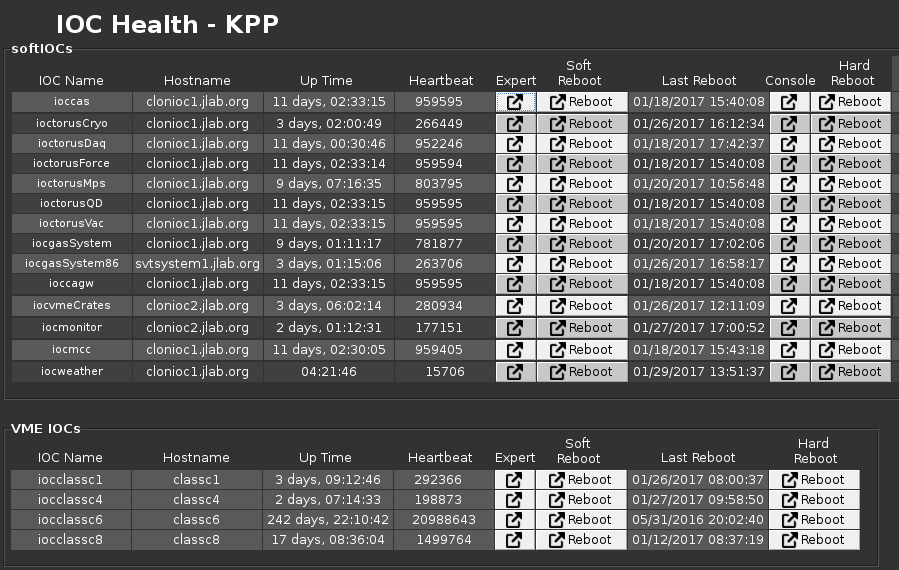
\includegraphics[width=\textwidth]{pics/iochealth-KPP}
  \caption{The primary IOC health screen for the KPP Run, showing uptime, heartbeats, and buttons to restart them.  \label{fig:iochealth}}
\end{figure}

\subsection{Motors}
The beamline devices in Hall B include encoderless stepping motors.  When their IOC is restarted, the actual motor stage position is unchanged (the motor does not move), but the software motor position is reset to zero.  If the motor was at a non-zero position during IOC reboot, then a recalibration is required in order for the motor position in EPICS to reflect the actual motor position.  The is generally the case for collimators and the beam stopper and viewer motors, because their normal position during running is non-zero.  The harps are generally left at zero when not in use and thus do not require recalibration unless in active use during the IOC reboot.  See Table~\ref{tab:stepmot} for a list of motors and their corresponding IOC.

\begin{table}[htpb]\centering
  \begin{tabular}{|c|c|} \hline
    \texttt{classc1} & \texttt{classc4} \\ \hline
    Collimator       & Beam Stopper \\
    Harp 2C21        & Beam Viewer \\
    Harp 2C24        & \\
    Harp 2H01        & \\
    M$\o$ller Target & \\ \hline
  \end{tabular}
  \caption{Stepping motors on two VME IOCs in Hall B.\label{tab:stepmot}}  
\end{table}

\section{High Voltage}
The largest controls system in Hall B in terms of number of channels is high voltage (HV), with over 20 CAEN mainframes including SY527, SY1527, and SY4527 models.  An overview screen of the status of all HV in Hall B is accessible from the HV button in the main CLAS12 menu as shown in Figure~\ref{fig:hv}.  Clicking on a detector in this overview screen will bring up the HV controls for that detector (also accessible under each detector's button in the main menu).

\begin{figure}[htbp]\centering
  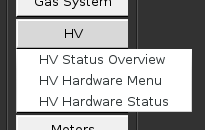
\includegraphics[width=0.3\textwidth]{pics/hvmenu}
  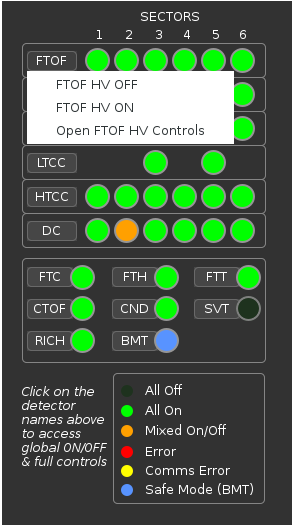
\includegraphics[width=0.2\textwidth]{pics/hvstat}
  \caption{Access to the HV overview screen from the main menu (left).  Clicking on a detector's name in the overview screen (right) will open its HV controls screen.\label{fig:hv}}
\end{figure}


\section{Strip Charts}
There are two applications available for plotting time histories of slow controls variables:  StripTool and MyaViewer.  Both are available from the {\em Strip Charts} button at the bottom of the main CLAS12 controls menu as shown in Figure~\ref{fig:strips}.

The suggested tool for online operations in Hall B is StripTool, which has no access to archived data but is very robust and stable.  MyaViewer is necessary for expert studies and can access the Mya archive used to store previous years of Hall B controls data.  In either case, configuration files are loadable from their user interfaces to view a predetermined set of variables, or else you can choose any process variable to plot.

\begin{figure}[htbp]\centering
    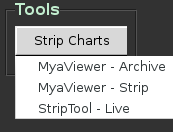
\includegraphics[width=0.2\textwidth]{pics/strips}
    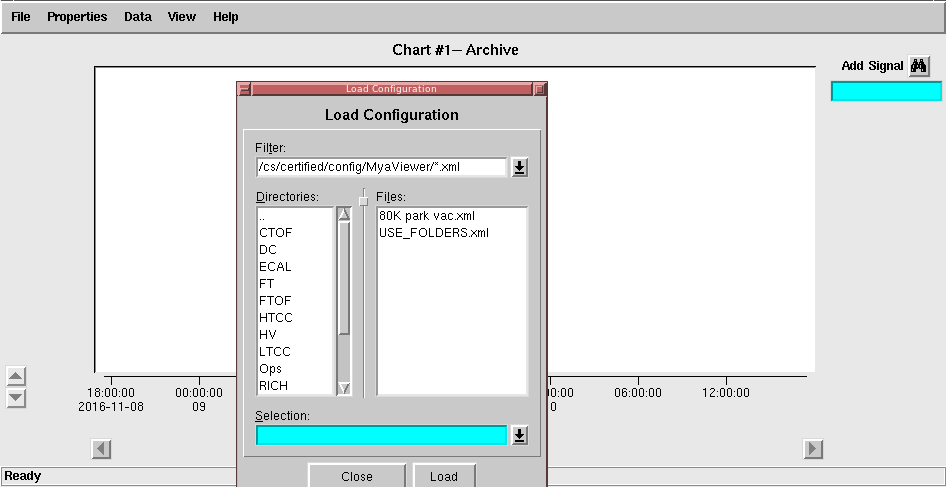
\includegraphics[width=0.7\textwidth]{pics/myaviewer}
    \caption{Utilities for plotting time histories of slow controls variables are accessible from the {\em Tools} section of the CLAS12 main menu (left).  An example of running MyaViewer and opening a preset configuration file via the {\em File $\rightarrow$ Load Config} menu is shown on right.\label{fig:strips}}
\end{figure}

\section{Logbook Entries and Screenshots}\label{sec:logentry}
We use the JLab logbook system, and the primary Hall B logbook is called HBLOG and accessible in a web browser at
\begin{center}\url{https://logbooks.jlab.org/book/HBLOG}\end{center}
In Hall B there are two primary methods for adding content to the logbook:
\begin{enumerate}
\item Use the web browser interface after logging in with your personal CUE credentials.  That is the normal method used for filling out the shift checklist, updating a shift summary log entry, following up with comments on previous log entries, or adding more complex log entries (e.g. with multiple images).
\item Use our Hall B GUI that facilitates taking screenshots and quickly sending one to the HBLOG logbook as \texttt{user=clasrun}.  This is accessed via the ``logbook entry'' item from the desktop menu, or via the following script in a terminal:
\begin{center}\texttt{logbookEntry.sh}\end{center}
    {\em This is also the preferred method for taking screenshots} and will always save them in \texttt{\$HOME/screenshots} with timestamped filenames.  See Figure~\ref{fig:logbookEntry} for details.
\end{enumerate}
    \begin{figure}[htbp]\centering
        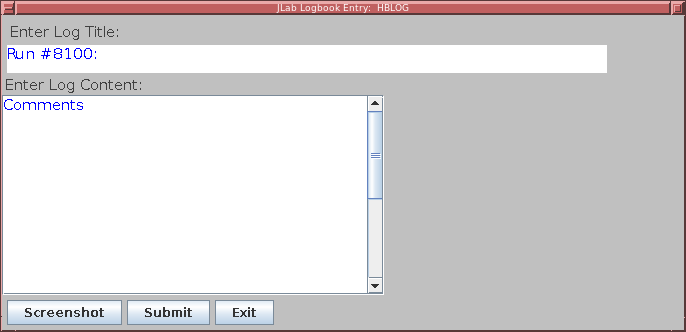
\includegraphics[width=0.49\textwidth]{pics/logbookEntry1.png}
        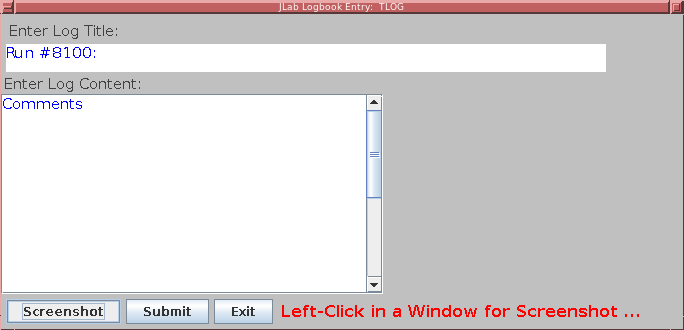
\includegraphics[width=0.49\textwidth]{pics/logbookEntry2.png}
        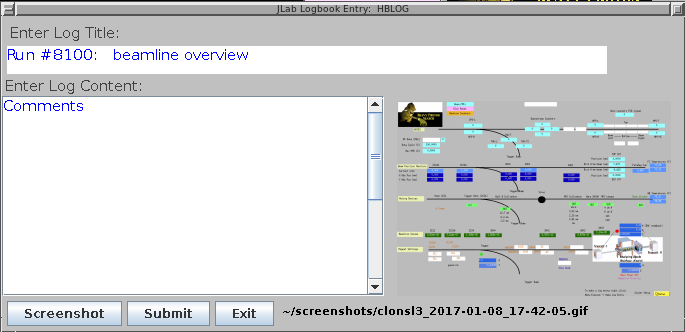
\includegraphics[width=0.49\textwidth]{pics/logbookEntry3.png}
        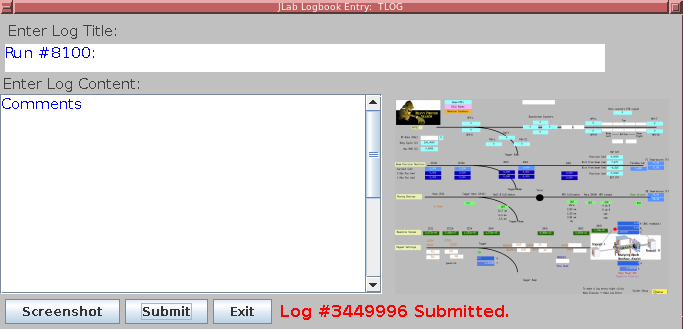
\includegraphics[width=0.49\textwidth]{pics/logbookEntry4.png}
        \caption{Upon first opening the logbook/screenshot GUI (top left), only the log title has been automatically initialized (with the current run number).  After clicking the ``Screenshot'' button (top right), it is waiting for you to left-click in the window you desire to capture (clicking the desktop instead of a window will capture the entire desktop).  After taking a screenshot (bottom left), a snapshot of the image and its filename on disk are automatically displayed.  Note that the ``Screenshot'' button can be used repeatedly to change the screenshot if you do not like the previous result, or just want to take more screenshots.  The ``Submit'' button can be used to generate an entry in the HBLOG logbook, and after success the entry number will be displayed (bottom right).\label{fig:logbookEntry}}
\end{figure}


\section{Paging System Experts}\label{sec:pagingexperts}
Paging on-call experts is available from the main CLAS12 controls menu via the {\em Page Experts} button at the very top of the screen (see Figure~\ref{fig:mainmenu}).  This will open a dropdown menu to choose the desired subsystem, and then open a new window in which to enter a message to be sent to the corresponding expert, as illustrated in Figure~\ref{fig:pageexpert}.
\begin{figure}[htbp]\centering
  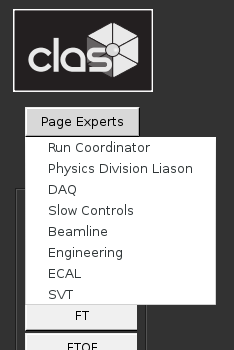
\includegraphics[width=0.2\textwidth]{pics/pageexpert}
  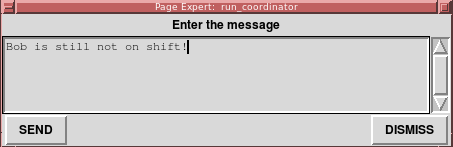
\includegraphics[width=0.6\textwidth]{pics/pageexpertmsg}
  \caption{The dropdown menu for choosing which expert to page (left) and the resulting dialog window in which to enter the message contents (right).\label{fig:pageexpert}}
\end{figure}

\newpage
\section{Slow Controls Contacts}
The individuals to be contacted for Hall B slow controls are shown in Table \ref{tab:experts}.  The first point of contact for shift operations is always the on-call controls expert, accessible from the paging system described in Section~\ref{sec:pagingexperts} of this document and the phone number in the first row of Table \ref{tab:experts}.  Additional contacts are listed in the table as a fallback.

\begin{table}[htbp]\centering
    \begin{tabular}{llcr}\toprule[1.5pt]
        On-Call & & \ \ \ \ \ 757-748-6922 & \\ \cmidrule[0.5pt]{1-4}
         & Nathan Baltzell & 757-259-5902 & \ \ \ \ \ \texttt{baltzell@jlab.org} \\
         General \ \ \ \ \       & Ken Livingston  &           & \texttt{kliv@jlab.org} \\
                & Wesley Moore & 757-259-6033 &  \texttt{wmoore@jlab.org} \\
                & Bryan McKinnon & & \texttt{mckinnon@jlab.org} \\
        \bottomrule[1.5pt]
    \end{tabular}
    \caption{Hall B slow controls contacts.\label{tab:experts}}
\end{table}

\section{Remote Usage}\label{sec:remote}
There are separate server-grade machines for remote controls access, all with access to the same software and running the same operating system as the desktops in the counting house.  For access outside the counting house, login to the server \texttt{clonsl2}.  {\bf\em In order to avoid heavly load on the machines used by counting house shift workers, it is important to not run on \texttt{clonpc} desktops remotely}.  All controls computers are behind JLab's \texttt{hallgw} gateway and require 2-factor authentication for remote access.  

\newpage
\section{Accelerator Screens}
The accelerator's screens are accessed from the main CLAS12 menu via the {\em JMenu} button (see Figure~\ref{fig:jmenu}).  This uses the \texttt{hbops} account on \texttt{hlbl00}, a machine owned and maintained by the accelerator group.  If a prompt requests a username, password, or terminal type, just press {\em Enter}.  The location of the button on the CLAS12 menu and the JMenu screen that should appear are shown in Figure~\ref{fig:jmenu}.

{\bf\em Note it is best to only have one instance of JMenu running.  Multiple instances have been known to result in frozen JMenus.}
\begin{figure}[htbp]\centering
  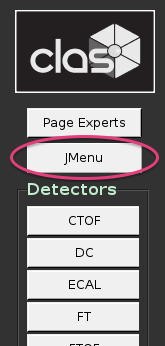
\includegraphics[width=0.16\textwidth]{pics/clas12jmenu}
  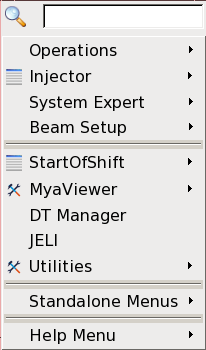
\includegraphics[width=0.2\textwidth]{pics/jmenu}
  \caption{The location of the button to access the accelerator screens from the CLAS12 controls menu (left) and the resulting accelerator JMenu main screen (right).\label{fig:jmenu}}
\end{figure}
    \subsection{Tagger}
To open the accelerator's controls for the Tagger magnet, from the main JMenu screen (Figure~\ref{fig:jmenu}) navigate:
\begin{center}{\em Operations $\to$ Magnets $\to$ Hall B Tagger}\end{center}
The tagger screen is shown in Figure~\ref{fig:tagger}.
    \subsection{FSD}
To open the accelerator's main screen for the fast shutdown system:
\begin{center}{\em Operations $\to$ FSD $\to$ FSD Overview (Multi-Tree)}\end{center}
From, there you can access the Hall B 2H001 FSD via:  
\begin{center}{\em 2H001 $\to$ Hall B HPS Halo Counters (new) (Collimator) $\to$ User Screen}\end{center}
The 2H001 FSD screens are shown in Figure~\ref{fig:fsd}
\begin{figure}[htbp]\centering
  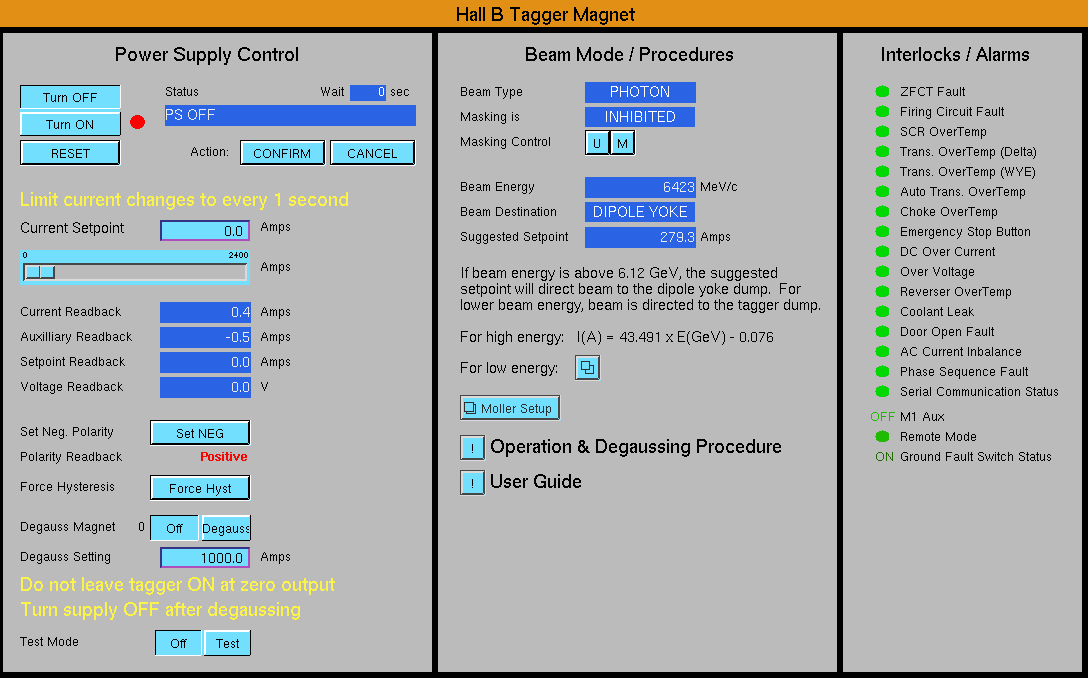
\includegraphics[width=0.88\textwidth]{pics/tagger}
  \caption{The accelerator's Hall B Tagger magnet controls.\label{fig:tagger}}
\end{figure}
\begin{figure}[htbp]\centering
  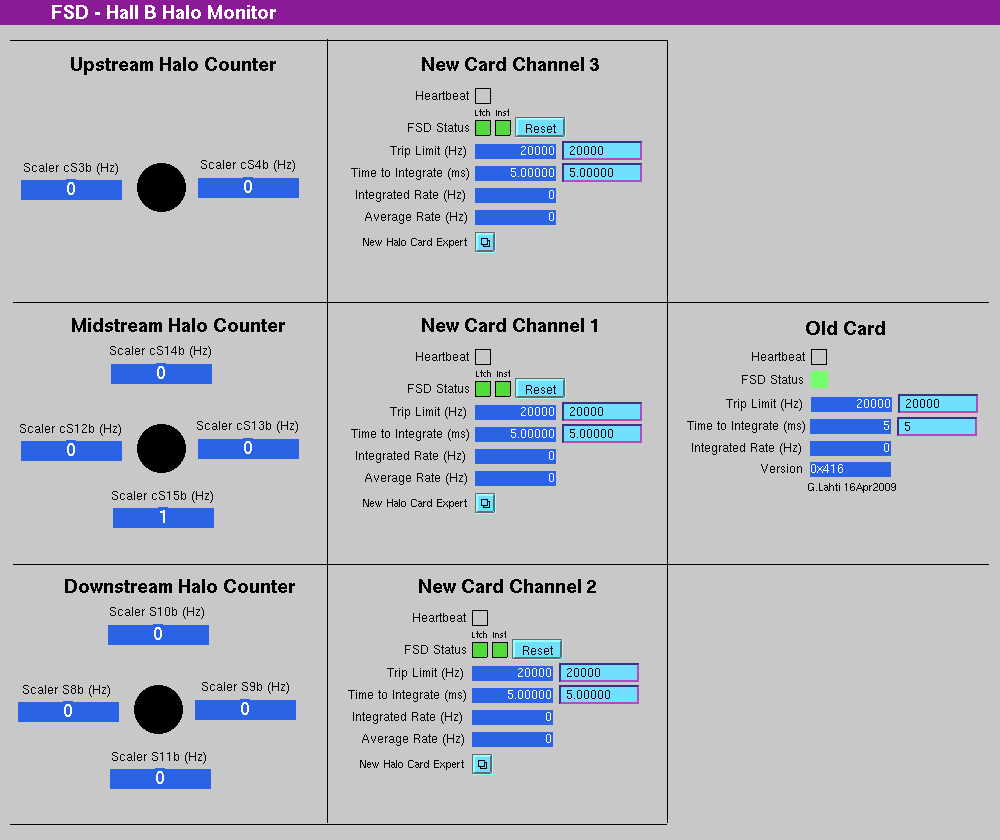
\includegraphics[width=0.88\textwidth]{pics/fsdexpert}\vspace{2mm}
    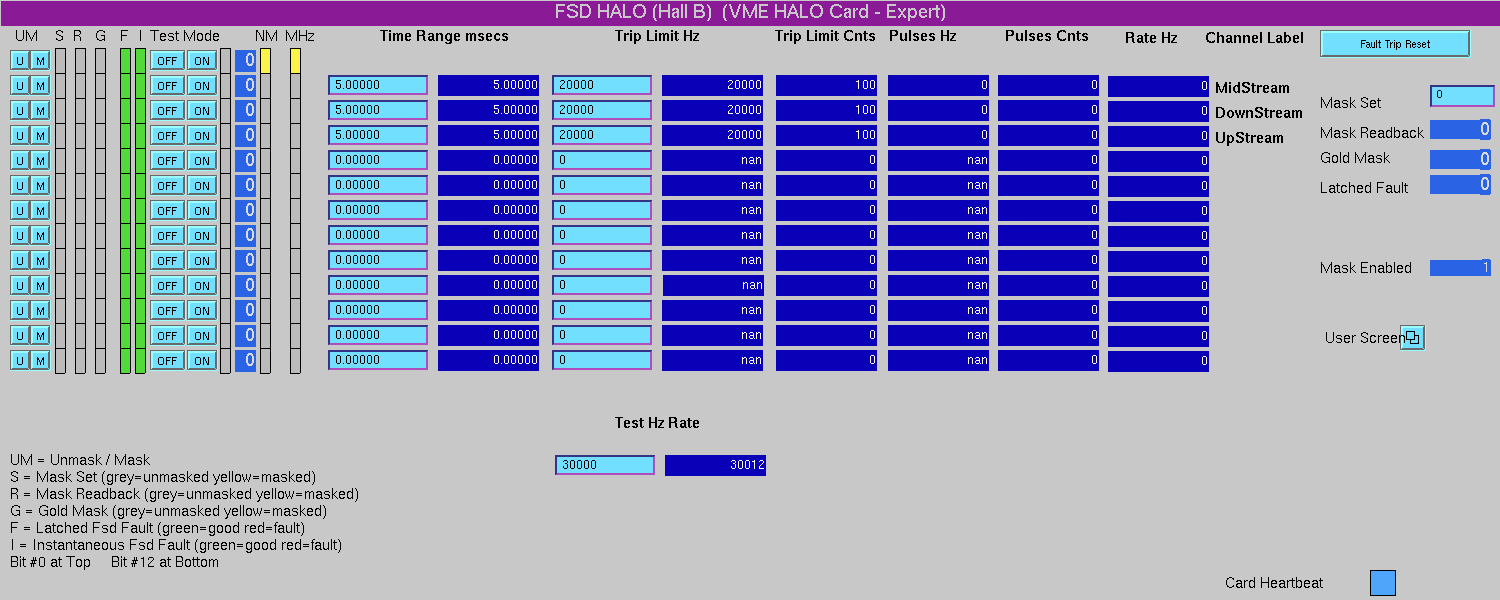
\includegraphics[width=0.88\textwidth]{pics/fsduser}
  \caption{The user (top) and expert (bottom) Hall B 2H001 FSD screens.\label{fig:fsd}}
\end{figure}
\subsection{Beam Viewers} The accelerators cameras are accessible from {\em JMenu} via  
\begin{center}{\em Operation $\to$ Viewers $\to$ Cross Point Switcher $\to$ Xpt Switcher}\end{center}
which opens the screen in Figure~\ref{fig:viewer}.  From there, the Hall B viewer is accessible via buttons:
\begin{center}$\to$ (``Hall B Video - Live'' button) ! $\to$ live BC4 (ffplay)\end{center}

\begin{figure}[htbp]\centering
  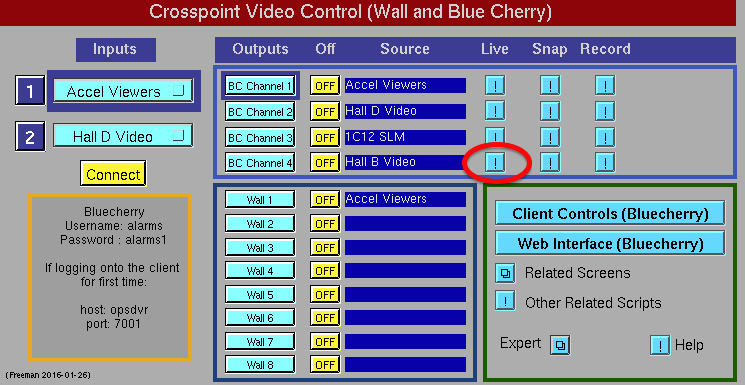
\includegraphics[width=0.88\textwidth]{pics/viewer}
  \caption{Access to the accelerator's live beam viewers.  The button for the Hall B viewer is circled in red.\label{fig:viewer}}
\end{figure}


%\bibliography{clas12slow_ops_shift}
\end{document}

